\documentclass{article}
\usepackage[utf8]{inputenc}

\usepackage{natbib}
\usepackage{graphicx}

% Drafting
\usepackage{xcolor,soul}
\usepackage{fullpage}
\usepackage{setspace}
\usepackage{blindtext}
\doublespacing

\definecolor{mwcolor}{HTML}{8af67d}
\definecolor{vgcolor}{HTML}{c88bff} % MPL purple
\definecolor{citecolor}{HTML}{c696f0} % MPL purple

% Tools for leaving todo notes around
\usepackage[colorinlistoftodos]{todonotes}
\newcommand{\citeme}[1]{%
  \todo[color=citecolor]{%
  \ifstrempty{#1}{[citation needed]}{[cite: #1]}%
  }%
}
\newcommand{\mw}[2]{%
  \sethlcolor{mwcolor}\hl{#2}\sethlcolor{yellow}%
  \ifstrempty{#1}{}{%
    \todo[color=mwcolor]{#1 [MW]}%
  }%                  
}
\newcommand{\vg}[2]{%
  \sethlcolor{vgcolor}\hl{#2}\sethlcolor{yellow}%
  \ifstrempty{#1}{}{%
    \todo[color=vgcolor]{#1 [VG]}%
  }%                  
}

\usepackage{authblk}

\title{Origin of Rapid Delithiation In Secondary Particles Of \nca{} and \nmc{} Cathodes}

\author[1,2,3]{Mark Wolfman}
\author[1]{Brian M.\ May}
\author[4]{Vishwas Goel}
\author[4]{Sicen Du}
\author[5,6]{Young-Sang Yu}
\author[7]{Nicholas V.\ Faenza}
\author[7]{Nathalie Pereira}
\author[8]{Antonin Grenier}
\author[3]{Kamila M.\ Wiaderek}
\author[3]{Ruqing Xu}
\author[9]{Jiajun Wang}
\author[8]{Karena W.\ Chapman}
\author[7]{Glenn G. Amatucci}
\author[4]{Katsuyo Thornton}
\author[1]{Jordi Cabana\thanks{Corresponding author: jcabana@uic.edu}}

\affil[1]{Department of Chemistry, University of Illinois at Chicago}
\affil[2]{Chemical Sciences and Engineering Division, Argonne National Laboratory}
\affil[3]{X-ray Science Division, Advanced Photon Source, Argonne National Laboratory}
\affil[4]{Department of Materials Science and Engineering, University of Michigan}
\affil[5]{Department of Physics, Chungbuk National University}
\affil[6]{Advanced Light Source, Lawrence Berkeley National Laboratory}
\affil[7]{Energy Storage Research Group, Department of Materials Science and Engineering, Rutgers, The State University of New Jersey}
\affil[8]{Department of Chemistry, Stony Brook University}
\affil[9]{Harbin Institute of Technology}

\date{}


\begin{document}

\maketitle

%%%%%%%%%%%%%%%%%%%%%%%
\section{Introduction}
%%%%%%%%%%%%%%%%%%%%%%%

\blindtext

%%%%%%%%%%%%%%%%%%
\section{Results}
%%%%%%%%%%%%%%%%%%

\begin{enumerate}
  \item Hello
\end{enumerate}

\begin{figure}
  \includegraphics[width=\textwidth]{ys-echem.png}
  \caption{SoCs for ex-situ bulk XANES.}
\end{figure}

\begin{figure}
  \includegraphics[width=\textwidth]{ys-xanes.png}
  \caption{How to judge SoC from Ni K-edge XANES. The trend between
    white line peak position and SoCs is not perfect linear, but we
    still can estimate the oxidation states of Ni.}
\end{figure}

\begin{figure}
  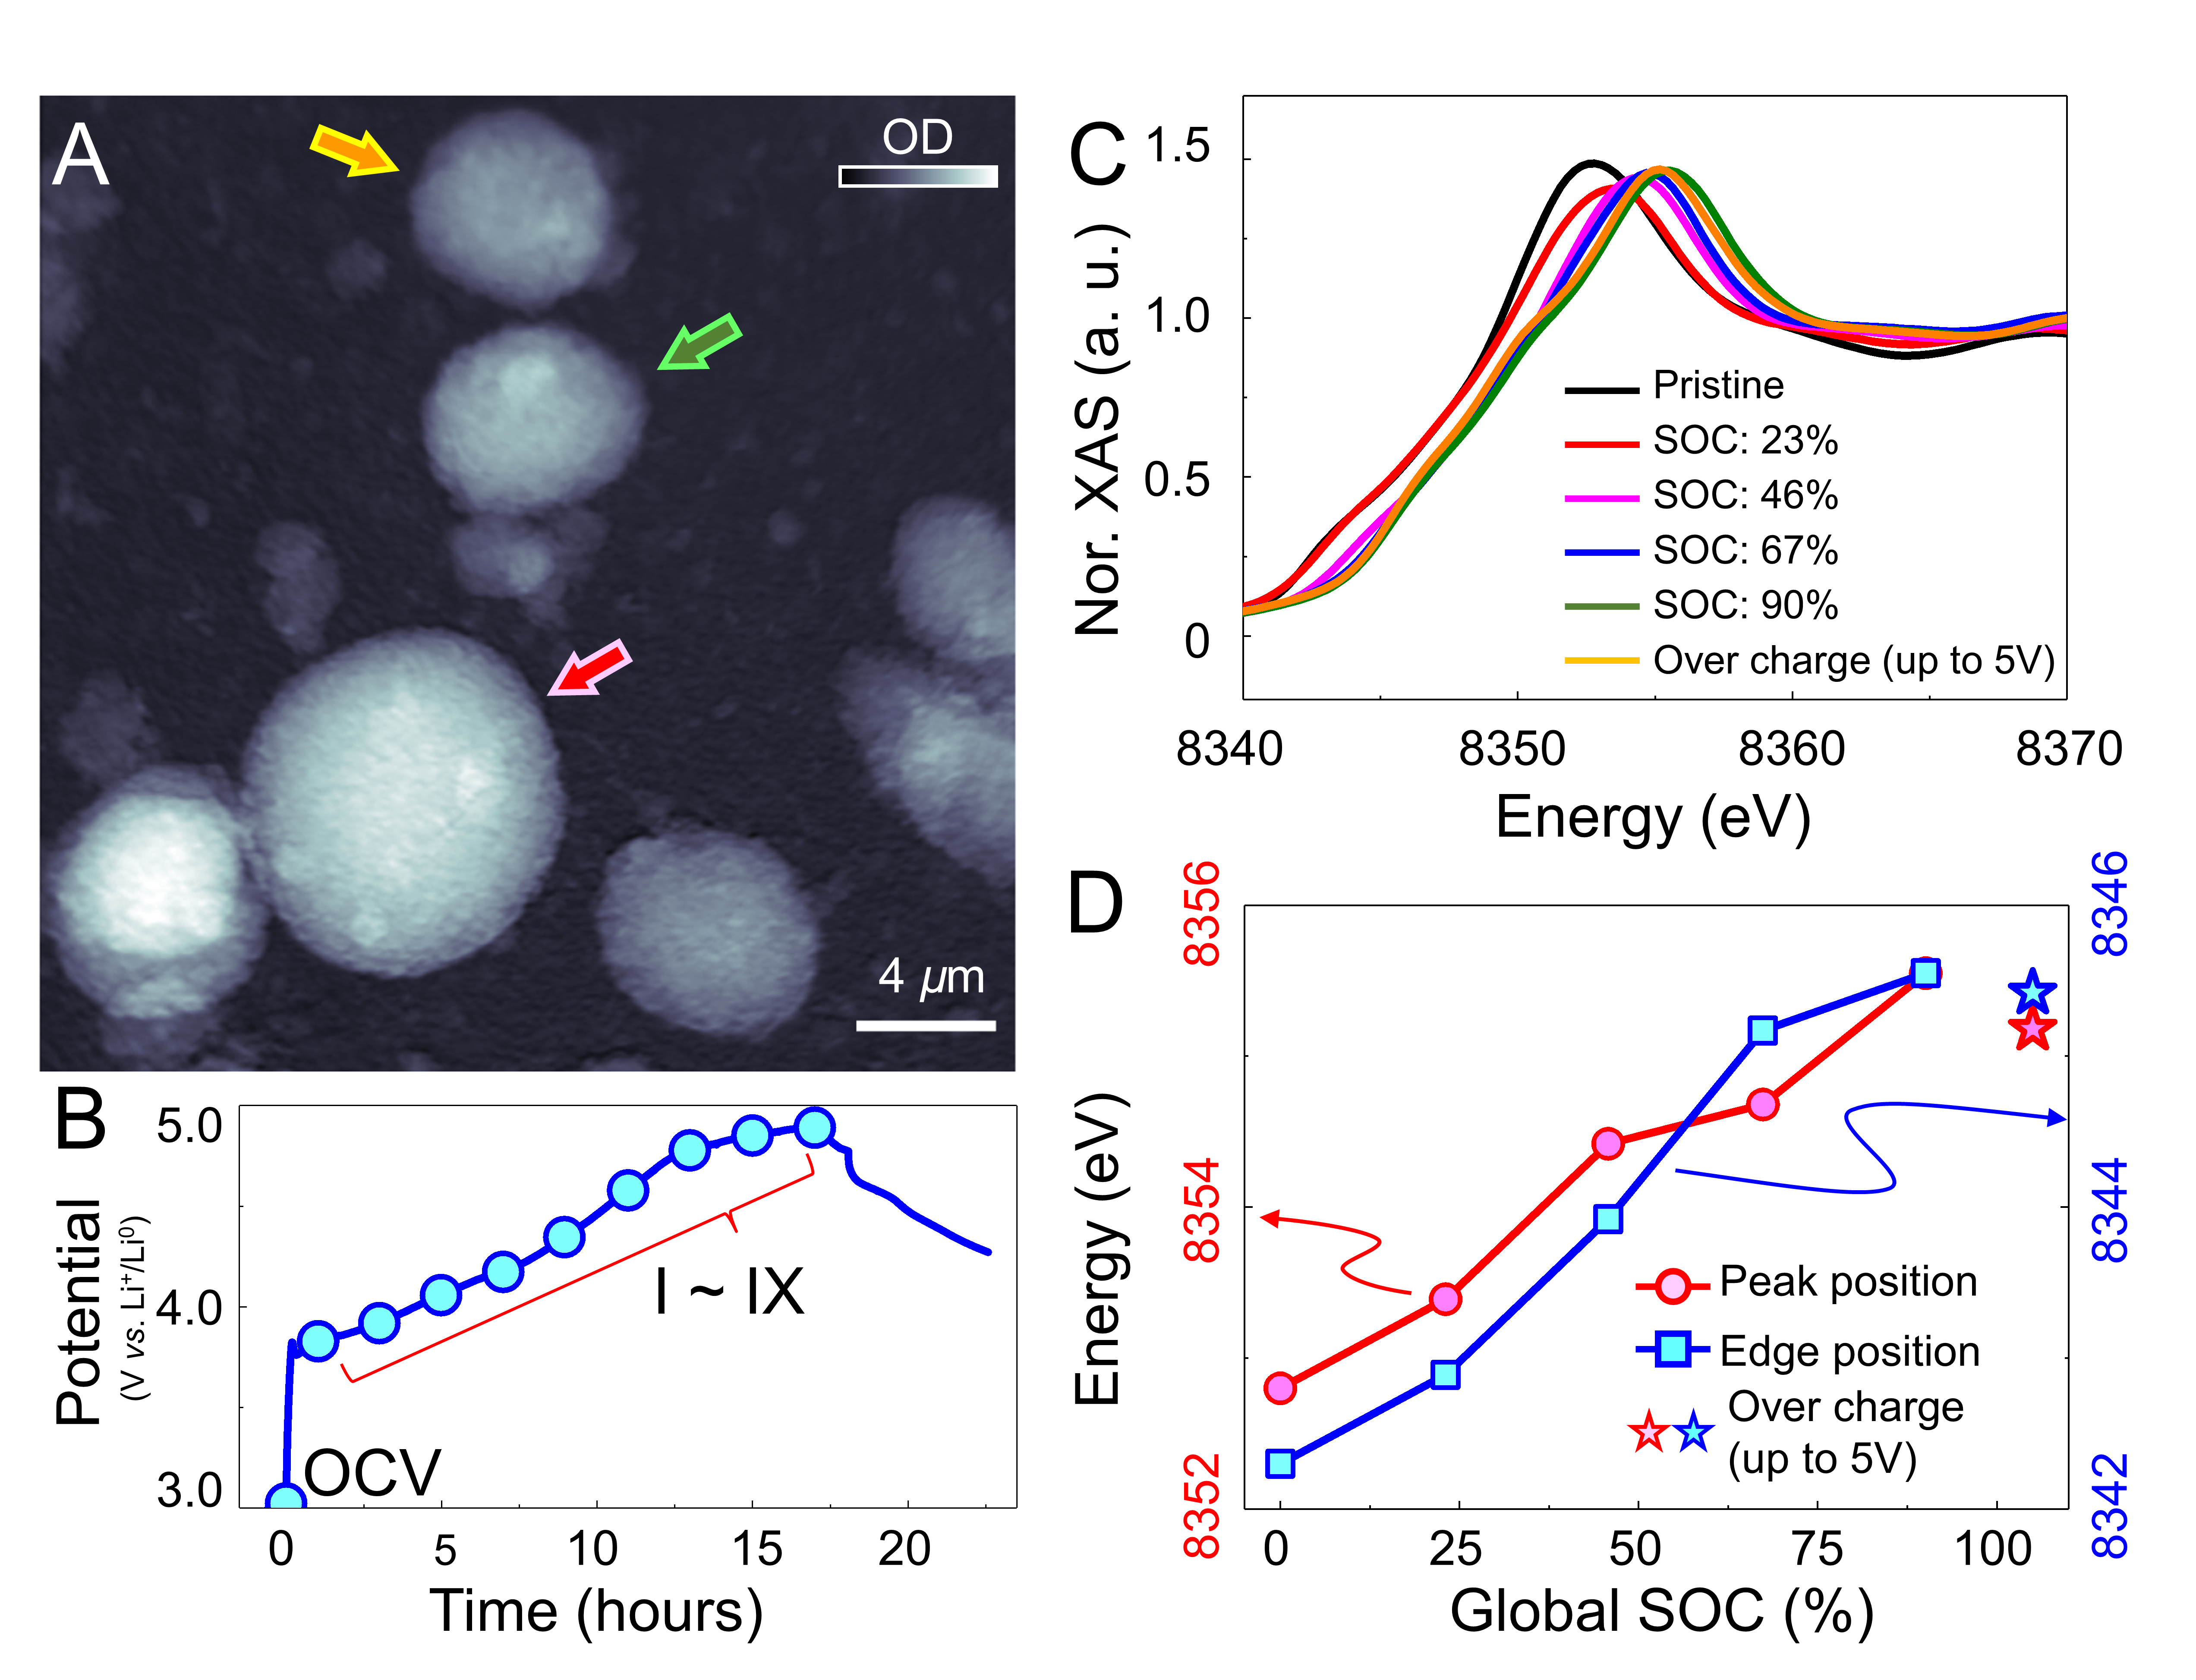
\includegraphics[width=\textwidth]{ys-xanes-fov.png}
  \caption{(A) Field-of-view (FoV) for in-situ hard X-ray full-filed
    transmission microscopy. (B) Electrochemical response of the
    in-situ cell. Identical FoV was repeatedly visualized (OCV \& SoC I
    ~ IX) during battery operation.}
\end{figure}

\begin{figure}
  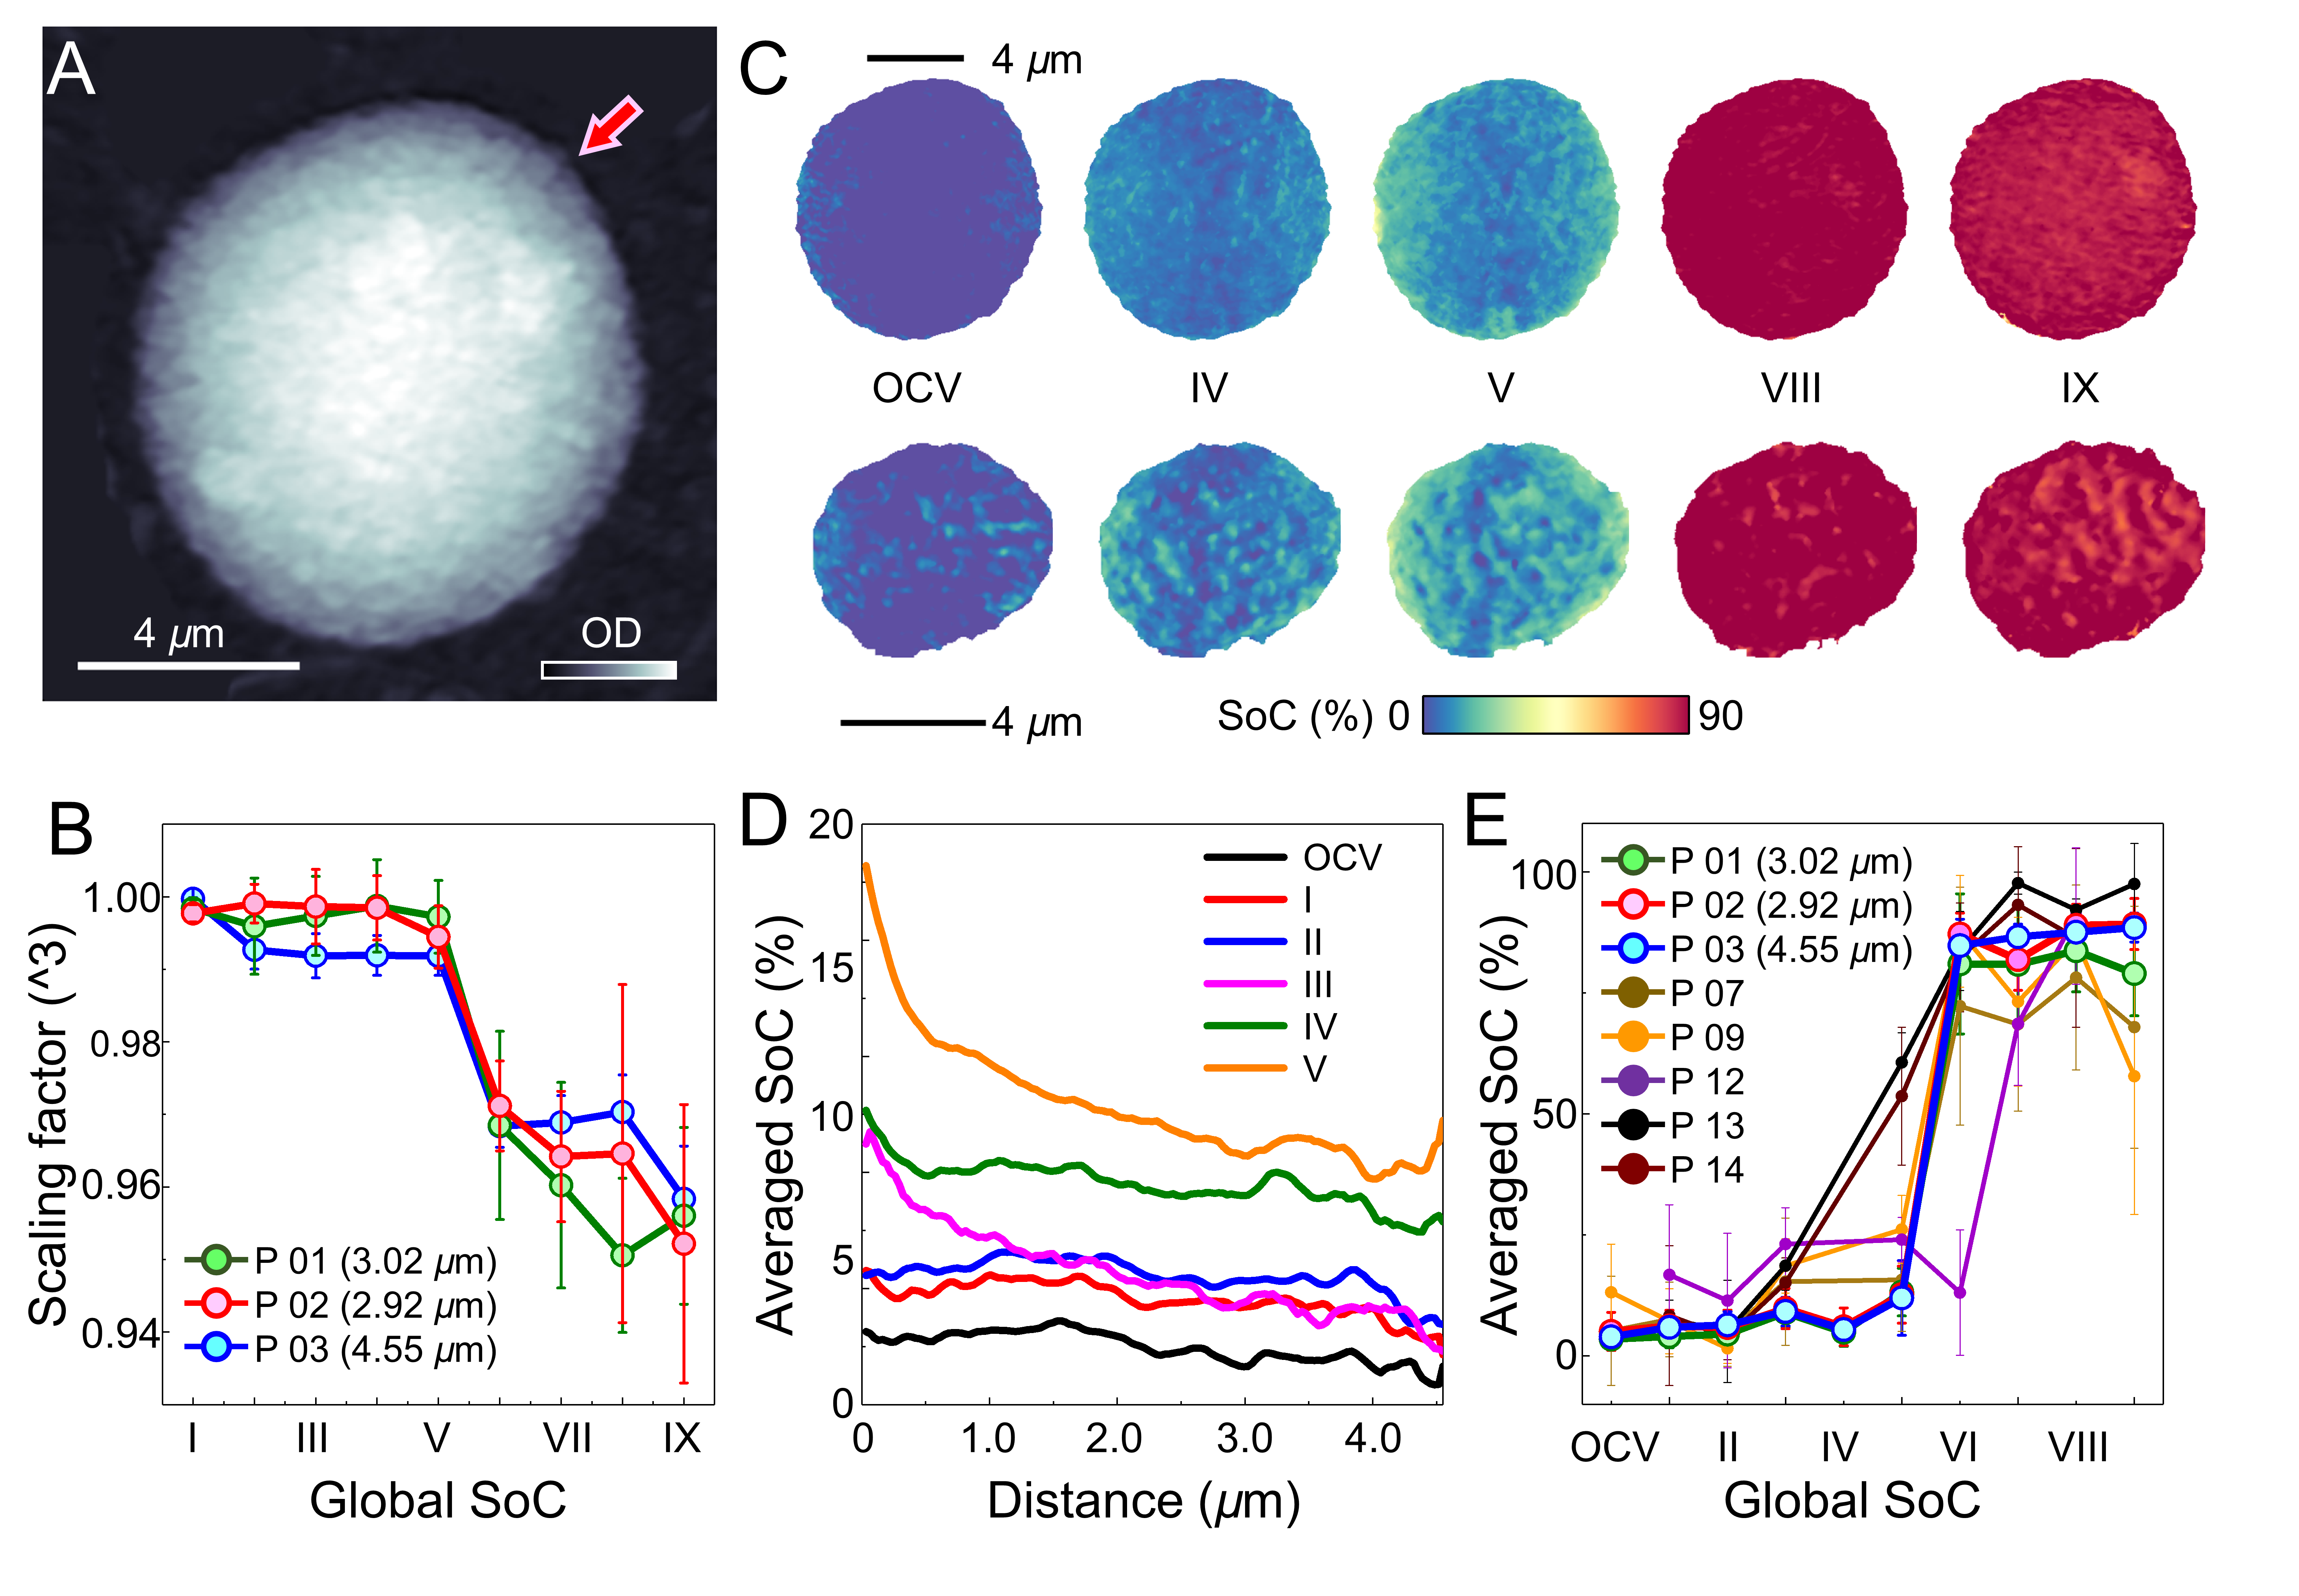
\includegraphics[width=\textwidth]{ys-soc-txm.png}
  \caption{See text}
  \label{ys-soc-txm}
\end{figure}

Figure \ref{ys-soc-txm}:

(A) Isolated 2nd particle in the FoV. The crack (indicated as red
arrow) suddenly appeared at the SoC VI (same sudden ``jumps'' position
in Jordi's e-mail). (B) Geometrical scaling factor with respect to
global SoCs. At ‘jump’ position, the volumes (1-dimensional scaling
factor \textasciicircum3) of the 2nd particles shrank around 3\%. The 1-dimensional
scaling factor was calculated by intensity-based image registration of
identical particles with respect to different SoCs. The enhance
robustness of analysis, 1-dimensional scaling factors were calculated
at all energy points (I don't remember exact the number of points but
it should be 30 ~ 40 points. Need to revisit the data) in imagespectra
and STD of the calculated 1-dimensional scaling factors\^{}3 shown as
error bars.  The shrinkage of the 2nd particles is smaller that
crystallographic volume shrinkage of the unit cell (I don't remember
exact number.) and cause the empty space inside (means microstructural
defaces such as void and crack).  (C) and (D) Chemical heterogeneity
of 2nd particle -> As Jordi mentioned, they are not the important
point. : )

(E) Averaged SoC of each 2nd particle with respect to global
SoCs. The positions of ``jump'' are differed.  The definition of
several SoC 1. Global SoC -> SoC of the entire in-situ cell (shown
in Figure 3B) 2. SoC or averaged SoC -> SoC of each individual 2nd
particle.

%%%%%%%%%%%%%%%%%%%%%
\section{Discussion}
%%%%%%%%%%%%%%%%%%%%%

\Blindtext

%%%%%%%%%%%%%%%%%%%%%%%%%%%%%%%%
\section{Materials and Methods}
%%%%%%%%%%%%%%%%%%%%%%%%%%%%%%%%

\blindtext

%%%%%%%%%%%%%%%%%%%%%
\section{Conclusion}
%%%%%%%%%%%%%%%%%%%%%

\blindtext

\end{document}
